\documentclass[a4paper, 12pt]{article}

\usepackage{amsmath} %Todos los paquetes de matematicas
\usepackage{amsthm}
\usepackage{mathtools}
\providecommand{\abs}[1]{\lvert#1\rvert}
\providecommand{\norm}[1]{\lVert#1\rVert}
\usepackage{yhmath}
\usepackage[utf8]{inputenc}
\usepackage[spanish]{babel}
\usepackage{wrapfig} %Figuras flotantes
\usepackage{parselines}
\usepackage{enumitem}
\usepackage{xcolor}
\usepackage{graphicx}
\graphicspath{{images/}}
\usepackage{subcaption}
\usepackage[left=2cm,right=2cm,top=2cm,bottom=2cm]{geometry}
\usepackage{eurosym} %Euro, de nada misniños

\theoremstyle{definition}
\newtheorem{ej}{Ejercicio}



\title{\textbf{Relación de ejercicios 1 EDIP}}
\author{Carlos García, Bora Goker, Javier Gómez,  \\ Ana Graciani, J.Alberto Hoces}
\date{2020/2021}

\setlength{\parindent}{0px}

\begin{document}

\maketitle

\begin{ej}
El número de hijos de las familias de una determinada barriada de una ciudad es una variable estadística de la que se conocen los siguientes datos:

\begin{table}[!h]

    \begin{tabular}{|c|c|c|c|}
    \hline
     \(x_i\) & \(n_i\) & \(N_i \) & \(f_i \)  \\ \hline
     \(0 \) & \(80 \) & & \(0.16 \)  \\ 
     \(1 \) & \(110 \) & & \\ 
     \(2 \) &  & \(320 \) &   \\ 
     \(3 \) & & & \(0.18 \)  \\ 
     \(4 \) & \(40 \) & &\\ 
     \(5 \) & & & \\ 
     \(6 \) & \(20 \) & & \\ 
     \hline
    \end{tabular}
  
\vspace*{-90pt}
    \begin{align*}
    n_i &: \text{frecuencias absolutas }\\
    N_i&: \text{frecuencias absolutas acumuladas} \\
    f_i&: \text{frecuencias relativas}
    \end{align*}
\end{table}
\bigskip
\textbf{Conceptos:}
\begin{center}
    \fbox{
    \begin{minipage}[h!]{1\linewidth}
    \begin{itemize}
        \item Población\label{poblacion}: Es el conjunto de unidades o elementos con alguna/s característica/s en común, sobre el que se desea obtener cierta información. En este caso las familias de una determinada barriada de una ciudad.
        \item Tamaño de la población: 500 familias.
        \item Variable estadística: Es toda propiedad que se desea estudiar en la población y que debe poder ser observada sobre todos y cada uno de los individuos que la componen. En este caso el número de hijos de cada familia.
        \item Modalidades: Es una de todas las formas posibles en que la característica estadística que se estudia puede presentarse en la población. Cada individuo solo puede presentar una modalidad. En el ejercicio son todas las distintas \(x_i\). En este caso son 0, 1, 2, 3, 4, 5, o 6 hijos.
    \end{itemize}
    \end{minipage}
    }
\end{center}

\newpage

\begin{enumerate}[label=\textit{\alph*})]
    \item Completar la tabla de frecuencias.
    
       En toda tabla de una variable estadística discreta (y siempre que las modalidades se puedan ordenar) podemos identificar: 
    \begin{center}
    \fbox{
    \begin{minipage}[h]{1\linewidth}
    \begin{itemize}
        \item Frecuencia absoluta del valor o modalidad \(x_i\) (\(n_i\)): Número total de individuos en la población que presenta dicho valor (modalidad). 
        \item Frecuencia relativa del valor o modalidad \(x_i\) (\(f_i\)): Proporción del número de individuos que presenta dicho valor (modalidad).
        \item Frecuencia absoluta acumulada del valor o modalidad \(x_i\) (\(N_i\)): Número de individuos que presentan un valor (modalidad) menor o igual que \(x_i\).
        \item Frecuencia relativa acumulada del valor o modalidad \(x_i\) (\(F_i\)): Proporción de individuos que presentan un valor (modalidad) menor o igual que \(x_i\).
    \end{itemize}
    \end{minipage}
    }
    \end{center}
    
    
    \begin{center}
    \begin{tabular}{|c|c|c|c|}
    \hline
     \(x_i\) & \(n_i\) & \(N_i \) & \(f_i \)  \\ \hline
     \(0 \) & \(80 \) & \color{blue} \(80 \) & \(0.16 \)  \\ 
     \(1 \) & \(110 \) & \color{blue} \(190 \) & \color{blue} \(0.22 \)\\ 
     \(2 \) & \color{blue} \(130 \)  & \(320 \) & \color{blue} \(0.26\) \\
     \(3 \) & \color{blue} \(90 \) & \color{blue} \(410 \) & \(0.18 \)  \\ 
     \(4 \) & \(40 \) & \color{blue} \(450 \) & \color{blue} \(0.08\)\\ 
     \(5 \) & \color{blue} \(30 \) & \color{blue} \(480 \) & \color{blue} \(0.06 \) \\ 
     \(6 \) & \(20 \) & \color{blue} \(500 \) & \color{blue} \(0.04 \) \\ 
     \hline
    \end{tabular}
    \qquad \(f_i = \frac{n_i}{n}\)
    \end{center}
    
    \item Representar la distribución mediante un diagrama de barras y la curva de distribución.
    
    \begin{center}
    \fbox{
    \begin{minipage}[h]{1\linewidth}
    \begin{itemize}
        \item Diagrama de barras: Se trata de una representación en un sistema de ejes cartesianos donde el eje de abscisas presenta los valores de la variable, y se trazan barras verticales con longitudes proporcionales a sus frecuencias (absolutas o relativas). 
        \item Es la función definida para cada número real, x, como la proporción de datos menores o iguales que \(x\). 
        \[
        f(x)= \left\{ \begin{array}{lcc}
             0 \hspace{0.3cm} \forall x < x_1  & & \\
             \dfrac{\sum_{j=1}^in_j}{n} = \sum_{j=1}^if_j = \dfrac{N_i}{n} = F_i \hspace{0.3cm} \forall x \hspace{0.2cm} / \hspace{0.2cm} x_i \leq x < x_{i+1} \\
             1 \hspace{0.2cm} \forall x \geq x_k
             \end{array}
   \right.
        \]
    \end{itemize}
    \end{minipage}
    }
    \end{center}
    
    \begin{figure}[h!]
        \centering
        \begin{subfigure}[b]{0.45\linewidth}
        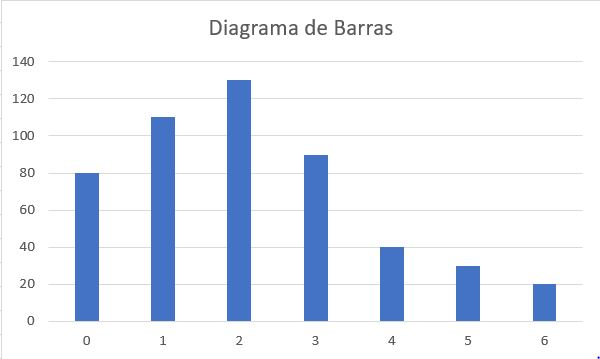
\includegraphics[width=\linewidth]{imagenes/Diagrama_barras_ejer1.JPG}
        \caption{Diagrama de barras}
        \end{subfigure}
        \begin{subfigure}[b]{0.45\linewidth}
        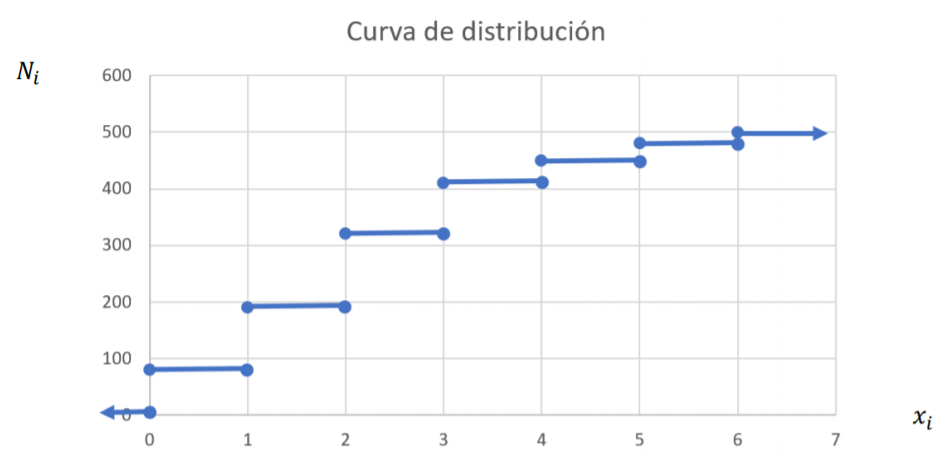
\includegraphics[width=\linewidth]{imagenes/Curva de distrubicon_ejer1.png}
        \caption{Curva de distribución}
        \end{subfigure}
    \end{figure}
    
    \newpage
    
    \item Promediar los valores de la variable mediante diferentes medidas. Interprétalas.
    
    \begin{center}
    \fbox{
    \begin{minipage}[h]{1\linewidth}
    \begin{itemize}
        \item Media: Medida de tendencia central que representa el valor promedio que más se ajusta a la distribución de los datos observados en la población.
        \item Mediana: Medida de posición que divide a los individuos de la población en dos efectivos iguales, supuestos ordenados por valor creciente del carácter.
        \item Moda: Medida de posición que determina la modalidad de mayor frecuencia (absoluta o relativa), la que más se repite.
    \end{itemize}
    \end{minipage}
    }
    \end{center}
    
    \begin{enumerate}[label=\textit{\roman*})]
        \item Media: Puesto que se pueden sumar el número de hijos y la media es única calculamos su media aritmética.
        
        \[
        \overline{x} =\frac{0\cdot80 + 1\cdot110 + 2\cdot130 + 3\cdot90 + 4\cdot40 + 5\cdot30 + 6\cdot20}{500} = 2.142 \hspace{0.1cm} \approx 2 \hspace{0.1cm} hijos
        \]
        
        \item Mediana:
        
        \[
            \frac{n}{2} = \frac{500}{2} = 250, \hspace{1cm} N_2 < 250 < N_3 \hspace{1cm} Mediana = 2 \hspace{0.2cm}hijos
        \]
        
        \item Moda:
        
        \[
            n_3 \geq n_j \hspace{1cm} \forall j \neq 3 \hspace{1cm} Moda = 2 \hspace{0.1cm} hijos
        \]
        
    \end{enumerate}
    
\end{enumerate}

\end{ej}

\begin{ej} 
La puntuación obtenida por 50 personas que se presentaron a una prueba de selección, sumadas las puntuación de distintos test, fueron:

\begin{center}
174, 185, 166, 176, 145, 166, 191, 175, 158, 156, 156, 187, 162, 172, 197, 181, 151, 161, 183, 172, 162, 147, 178, 176, 141, 170, 171, 158, 184, 173, 169, 162, 172, 181, 187, 177, 164, 171, 193, 183, 173, 179, 188, 179, 167, 178, 180, 168, 148, 173.
\end{center}

En este ejercicio estamos ante el estudio de una variable estadística discreta, por lo que hay nuevos añadidos a la tabla y por lo tanto, \textbf{nuevos conceptos}:

\begin{center}
    \fbox{
    \begin{minipage}[h]{1\linewidth}
    \begin{itemize}
        \item Marca de clase \(c_i\): Es el centro del intervalo de clase \(I_i\) y su valor es el que se tiene en cuenta a la hora de trabajar con los datos del intervalo \(I_i\), es decir, todos los datos se suponen idénticos a la marca de clase.
        \item Densidad de frecuencia \(h_i\): Valor numérico que indica el número de individuos que se hallan en un intervalo de clase \(I_i\) por unidad de amplitud \(a_i\).
        \item Amplitud \(a_i\): Diferencia entre los extremos superior e inferior de un intervalo de clase.
    \end{itemize}
    \end{minipage}
    }
    \end{center}
    
    Por otro lado, además, podemos identificar otros elementos definidos anteriormente:
    \begin{center}
    \fbox{
    \begin{minipage}[h]{1\linewidth}
    \begin{itemize}
        \item Población: personas que se presentaron a dicha prueba de selección.
        \item Tamaño de la población: 50 personas.
        \item Variable estadística: la nota que obtuvo el participante sumando todos los test de la prueba.
        \item En este caso todas las notas que se presentan en el enunciado, tomando en cuenta solo una de las apariciones que pueda hacer dicha nota.
    \end{itemize}
    \end{minipage}
    }
    \end{center}

\begin{enumerate}[label=\textit{\alph*)}]

\item Agrupar los datos en intervalos de amplitud 5 desde 140 a 200 y dar la tabla de frecuencias.

\begin{center}
    
\begin{tabular}{|c|c|c|c|c|c|c|c|}
    \hline
    \(I_i\) & \(n_i\) & \(N_i\) & \(f_i\) & \(F_i\) & \(c_i\) & \(a_i\) & \(h_i\) \\ 
    \hline
    \([140,145]\) & \(2\) & \(2\) & \(2/50\) & \(2/50\) & \(142.5\) & \(5\) & \(2/5\) \\
    \((145,150]\) & \(2\) & \(4\) & \(2/50\) & \(4/50\) & \(147.5\) & \(5\) & \(2/5\) \\
    \((150, 155]\) & \(1\) & \(5\) & \(1/50\) & \(5/50\) & \(152.5\) & \(5\) & \(1/5\) \\
    \((155,160]\) & \(4\) & \(9\) & \(4/50\) & \(9/50\) & \(157.5\) & \(5\) & \(4/5\) \\
    \((160,165]\) & \(5\) & \(14\) & \(5/50\) & \(14/50\) & \(162.5\) & \(5\) & \(5/5\) \\
    \((165,170]\) & \(6\) & \(20\) & \(6/50\) & \(20/50\) & \(167.5\) & \(5\) & \(6/5\) \\
    \((170,150]\) & \(10\) & \(30\) & \(10/50\) & \(30/50\) & \(172.5\) & \(5\) & \(10/5\) \\
    \((175,180]\) & \(8\) & \(38\) & \(8/50\) & \(38/50\) & \(177.5\) & \(5\) & \(8/5\) \\
    \((180,185]\) & \(6\) & \(44\) & \(6/50\) & \(44/50\) & \(182.5\) & \(5\) & \(6/5\) \\
    \((185,190]\) & \(3\) & \(47\) & \(3/50\) & \(47/50\) & \(187.5\) & \(5\) & \(3/5\) \\
    \((190,195]\) & \(2\) & \(49\) & \(2/50\) & \(49/50\) & \(192.5\) & \(5\) & \(2/5\) \\
    \((195,200]\) & \(1\) & \(50\) & \(1/50\) & \(50/50\) & \(197.5\) & \(5\) & \(1/5\) \\
    \hline
    & \(50\) & & \(1\) & & & & \\
    \hline
\end{tabular}

\end{center}


\newpage
\item
Representar la distribución mediante un histograma, poligonal de frecuencias y curva de distribución.\\
\begin{figure}[h!]
        \centering
        \begin{subfigure}[b]{0.45\linewidth}
        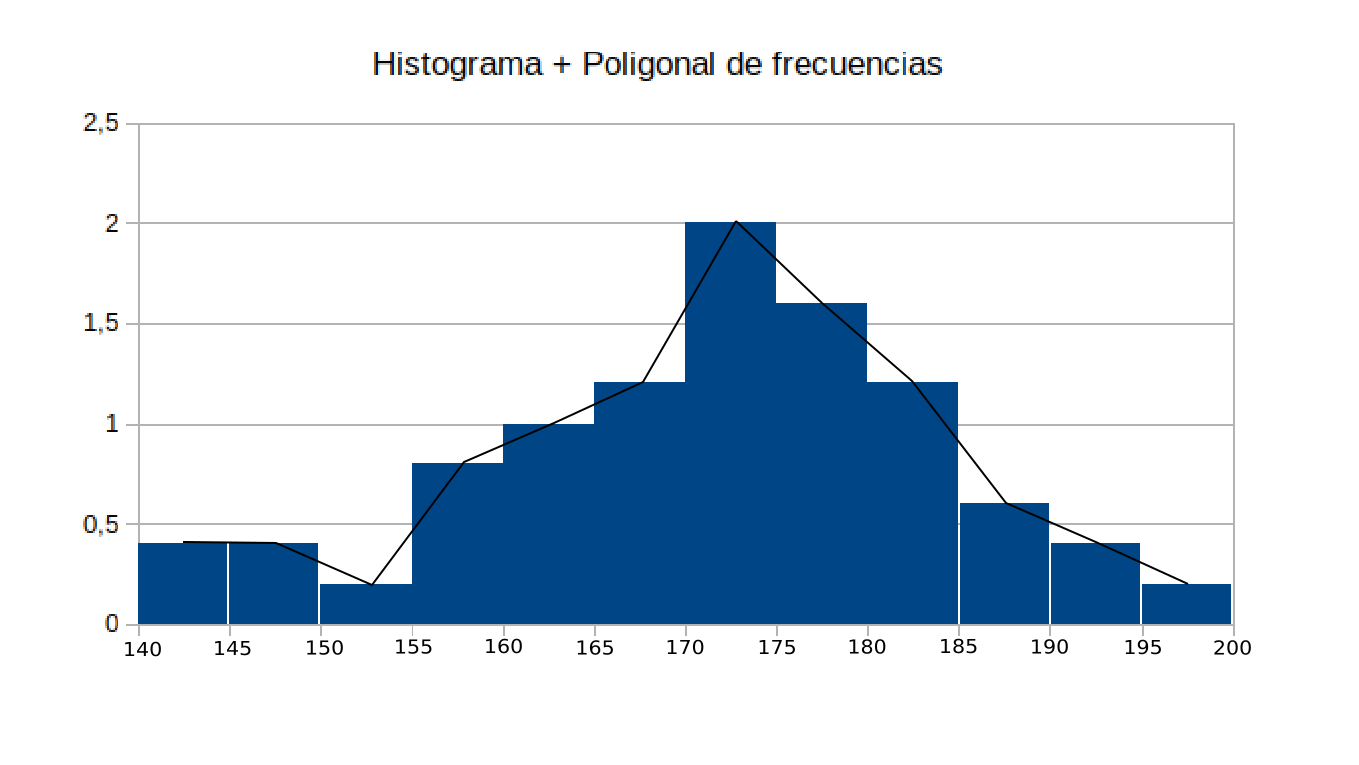
\includegraphics[width=\linewidth]{imagenes/Histograma_Ej_2.png}
        \caption{Histograma}
        \end{subfigure}
        \begin{subfigure}[b]{0.45\linewidth}
        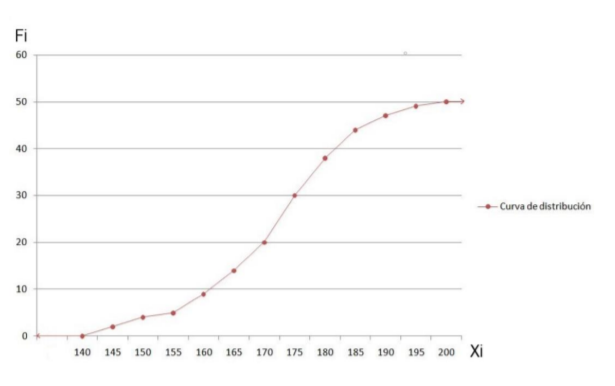
\includegraphics[width=\linewidth]{imagenes/Curva de distrubicon_ejer2.png}
        \caption{Curva de distribución}
        \end{subfigure}
    \end{figure}
\end{enumerate}
\end{ej}


\begin{ej}
La distribución de la renta familiar en el año 2003 por comunidades autónomas se recoge en la siguiente tabla:

\begin{table}[!h]

    \begin{tabular}{|c|c|c|c|c|c|c|c|}
    \hline
     \(I_i\) & \(n_i\) & \(N_i \) & \(f_i \) & \(F_i\) & \(c_i\) & \(a_i\) & \(h_i\)  \\ \hline
     \([8300, 9300] \) & \(2 \) & & & & & &\\ 
     \(,10200] \) & & \(5 \) & & & & & \\ 
     & & & & \(10/18 \)  & & \(1100 \) &   \\ 
     & & & \(2/18 \) & & \(1200 \) & &  \\ 
     & \(4 \) & & & & & & \(0.005/18\) \\ 
     & & \(18 \) & & & & & \(0.002/18\) \\ 
     \hline
    \end{tabular}
  
\vspace*{-130pt}
    \begin{align*}
   \hspace{12.5cm} 
    n_i&: \text{frecuencias absolutas }\\
    N_i&: \text{frec. absolutas acumuladas} \\
    f_i&: \text{frecuencias relativas} \\ 
    F_i&: \text{frec. relativas acumuladas} \\
    c_i&: \text{marcas de clase} \\
    a_i&: \text{amplitudes} \\
    h_i&: \text{densiades de frecuencia}
    \end{align*}
\end{table}

\begin{center}
    \fbox{
    \begin{minipage}[h!]{1\linewidth}
    \begin{itemize}
        \item Población: En este caso el conjunto de comunidades autónomas de España, y tomando en cuenta a Ceuta y Melilla como una comunidad extra.
        \item Tamaño de la población: 18 comunidades.
        \item Variable estadística: la renta familiar media en 2003 de cada comunidad autónoma.
        \item Modalidades: son los intervalos de la renta familiar media en 2003 por comunidad autónoma, es decir, 6 modalidades que van desde los 8300 \euro \hspace{0.07cm} hasta los 14500 \euro.
    \end{itemize}
    \end{minipage}
    }
\end{center}

\(\ast\) \textit{Cabe mencionar que el enunciado de este ejercicio no es del todo preciso, primero porque el número de comunidades autónomas que componen el Estado Español es 17 no 18 (de ahí que se considere a Ceuta y Melilla) y además la variable que se ha medido se supone que es le renta familiar \textbf{media} de las familias no la renta familiar a secas.} 

\begin{enumerate}[label=\textit{\alph*)}]
    \item Completar la tabla.
    
    \begin{center}
    \begin{tabular}{|c|c|c|c|c|c|c|c|}
    \hline
     \(I_i\) & \(n_i\) & \(N_i \) & \(f_i \) & \(F_i\) & \(c_i\) & \(a_i\) & \(h_i\)  \\ \hline
     \([8300, 9300] \) & \(2 \) & \color{blue} \(2 \) & \color{blue} \(0.11 \) & \color{blue} \(0.11 \) & \color{blue} \(8800 \) & \color{blue} \(1000 \) & \color{blue} \(0.002/18 \) \\ 
     \(\color{blue} (9300 \) \(,10200] \) & \(\color{blue} 3 \) & \(5 \) & \(\color{blue} 3/18 \) & \(\color{blue} 5/18 \) & \(\color{blue} 9750 \) & \(\color{blue} 900 \) & \(\color{blue} 0.00\wideparen{3}/18 \) \\
     \(\color{blue} (10200, 11300] \) & \(\color{blue} 5 \) & \(\color{blue} 10 \) & \(\color{blue} 5/18 \) & \(10/18 \)  & \(\color{blue} 10750 \) & \(1100 \) & \(\color{blue} 0.00\wideparen{45}/18 \)   \\ 
     \(\color{blue} (11300, 12700] \) & \(\color{blue} 2 \) & \(\color{blue} 12 \) & \(2/18 \) & \(\color{blue} 12/18 \) & \(12000 \) & \(\color{blue} 1400 \) & \(\color{blue} 0.0014/18 \)  \\ 
     \(\color{blue} (12700, 13500] \) & \(4 \) & \(\color{blue} 16 \) & \(\color{blue} 4/18 \) & \(\color{blue} 16/18 \) & \(\color{blue} 13100 \) & \(\color{blue} 800 \) & \(0.005/18\) \\ 
     \(\color{blue} (13500, 14500] \) & \(\color{blue} 2 \) & \(18 \) & \(\color{blue} 2/18 \) & \(\color{blue} 18/18 \) & \(\color{blue} 14000 \) & \(\color{blue} 1000 \) & \(0.002/18\) \\ 
     \hline
    \end{tabular}
    \end{center}
    
    \newpage
    
    \item Representar la distribución mediante un histograma, poligonal de frecuencias y curva de distribución.
    
    \begin{figure}[h!]
        \centering
        \begin{subfigure}[b]{0.45\linewidth}
        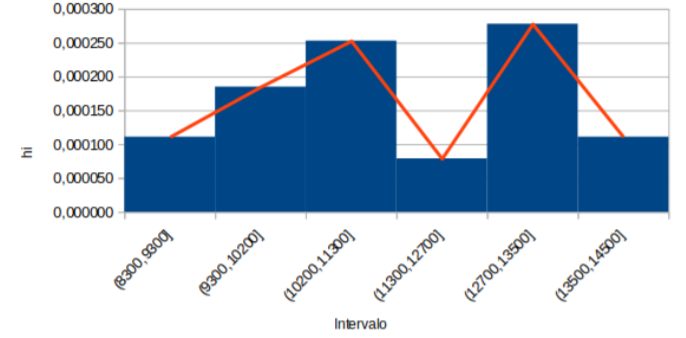
\includegraphics[width=\linewidth]{imagenes/Histograma_ejer_3.png}
        \caption{Histograma y poligonal de frecuencias}
        \end{subfigure}
        \begin{subfigure}[b]{0.45\linewidth}
        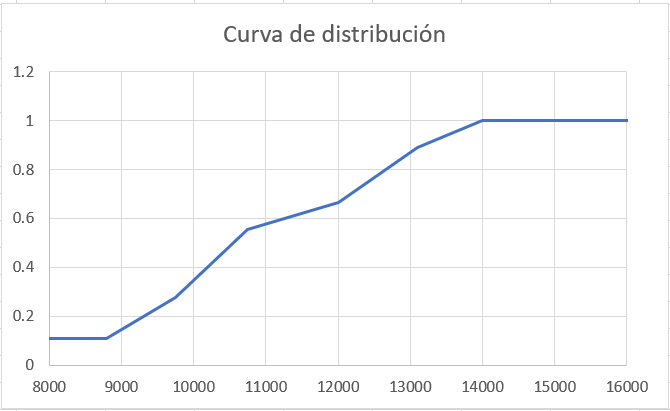
\includegraphics[width=\linewidth]{imagenes/Curva de distrubicon_ejer3.png}
        \caption{Curva de distribución}
        \end{subfigure}
    \end{figure}
    
    \item ¿Cuántas comunidades presentan una renta menor o igual que 12700 euros? ¿Y cuántas superior a 11300 euros?
    
    \(N_4 = 12 ; \qquad I_4 = (11300,12700] \) \newline
    12 comunidades presentan una renta menor o igual a 12700 \textup{\euro} .
    
    \(n_4 + n_5 + n_6 = 8\) \newline
    8 comunidades presentan una renta superior a 11300 \textup{\euro}.
    
\end{enumerate}


\end{ej}

\begin{ej}
En una determinada empresa se realiza un estudio sobre la calidad de su producción. La distribución siguiente informa sobre el número de piezas defectuosas encontradas en 100 cajas examinadas con 50 unidades cada una de ellas:

\begin{center}
    \begin{tabular}{|c|c|c|c|c|c|c|c|c|c|c|c|}
    \hline
     Nº piezas defectuosas & \(0\) & \(1\) & \(2\) & \(3\) & \(4\) & \(5\) & \(6\) & \(7\) & \(8\) & \(9\) & \(10\) \\
     \hline
     Nº de cajas & \(6\) & \(9\) & \(10\) & \(11\) & \(14\) & \(16\) & \(16\) & \(9\) & \(4\) & \(3\) & \(2\) \\
     \hline
    \end{tabular}
    
\end{center}

\begin{center}
    \fbox{
    \begin{minipage}[h!]{1\linewidth}
    \begin{itemize}
        \item Población: las cajas de una empresa con 50 piezas cada una de ellas.
        \item Tamaño de la población: 100 cajas.
        \item Variable estadística: el número de piezas defectuosas por caja estudiada.
        \item Modalidades: en este caso, 11 modalidades. Desde 0 hasta 10 piezas defectuosas, ambas inclusive.
    \end{itemize}
    \end{minipage}
    }
\end{center}

\begin{enumerate}[label=\textit{\alph*)}]
    \item Calcular el número medio de piezas defectuosas por caja.
    
    \[
    \overline{x} = \frac{1}{n} \sum_{i=1}^{k}n_ix_i = \frac{1}{100} \cdot 436 = 4.36 \hspace{0.3cm} piezas \hspace{0.2cm} defectuosas.
    \]
    
    \begin{center}
    \begin{tabular}{|c|c|c|c|c|c|c|}
    \hline
    \(x_i\) & \(n_i\) & \(n_i x_i\) & \(N_i\) & \(\abs{x_i -\overline{x}} n_i\) & \(\abs{x_i - Me} n_i\) & \(x_i^2 n_i\) \\
    \hline
    0 & 6 & 0 & 6 & \(26.16\) & 27 & 0 \\ 
    1 & 9 & 9 & 15 & \(30.24\) & \(31.5\) & 9 \\
    2 & 10 & 20 & 25 & \(23.6\) & 25 & 40 \\
    3 & 11 & 33 & 36 & \(14.96\) & \(16.5\) & 99 \\
    4 & 14 & 56 & 50 & \(5.04\) & 7 & 224 \\
    5 & 16 & 80 & 66 & \(10.24\) & 8 & 400 \\
    6 & 16 & 96 & 82 & \(26.24\) & 24 & 576 \\ 
    7 & 9 & 63 & 91 & \(23.76\) & \(22.5\) & 441 \\
    8 & 4 & 32 & 95 & \(14.56\) & 14 & 256 \\
    9 & 3 & 27 & 98 & \(13.92\) & \(13.5\) & 243 \\
    10 & 2 & 20 & 100 & \(11.28\) & 11 & 200 \\
    \hline
    & 100 & 436 & & 200 & 200 & 2488 \\
    \hline
    \end{tabular}
        
    \end{center}
    
    \item ¿Cuántas piezas defectuosas se encuentran más frecuentemente en las cajas examinadas?
    
    La moda de una distribución es el valor de mayor frecuencia (el más repetido). En este caso :
    \[
    n_6 = n_7 = 16 \hspace{1cm} M_o = x_6 = 5 \hspace{0.2cm} piezas \hspace{0.1cm} defectuosas \hspace{1cm} M_o = x_7 = 6 \hspace{0.2cm} piezas \hspace{0.1cm} defectuosas
    \]
    Podemos observar que nos hayamos ante una distribución bimodal.
    \item ¿Cuál es el número mediano de piezas defectuosas por caja?
    Recordemos que la mediana de una distribución es un valor que divide a los individuos de la población en dos efectivos iguales, supuestos ordenados por el valor creciente del carácter.
    
    
    \(x_i\quad/\quad N_{i-1} < \frac{n}{2} \leq N_i \rightarrow N_i = \frac{n}{2}; \quad Me = \frac{x_i+x_{i+1}}{2}=\frac{4+5}{2} = 4.5 \) piezas defectuosas
    
    \item Calcular los cuartiles de la distribución.  Interpretarlos.
    
    \begin{center}
    \fbox{
    \begin{minipage}[h!]{1\linewidth}
    \begin{itemize}
        \item Percentil: Es un valor, \(P_r \) \((r=1,\dotsc,100)\), que divide al conjunto ordenado de datos en dos partes, tales que el \(r \%\)  del total son inferiores o iguales a \(P_r\).
        \item Cuartiles: \(Q_1, Q_2, Q_3\) que equivalen a los percentiles de orden 25, 50 y 75 respectivamente.
    \end{itemize}
    \end{minipage}
    }
    \end{center}
    
    
    \(x_i\quad/\quad N_{i-1} <\frac{nr}{100} \leq N_i\).
    
    \begin{enumerate}[label=]
    \item \(Q_1 = P_{25} \quad \Rightarrow \quad x_i\quad/\quad N_{i-1} <\frac{n}{4} = 25 \leq N_i\).
    
    Como en este caso, \(N_3 = 25\), hemos de hacer la media aritmética entre \(x_3\) y \(x_4\).
    
    \(Q_1 = \frac{2+3}{2} = 2.5 \Rightarrow\) 25 \% de las cajas presentan \(3.5\) piezas defectuosas o menos. \\
    \item \(Q_2 = P_{50} = Me = 4.5 \Rightarrow\) El 50 \% de las cajas presentan 4.5 piezas defectuosas o menos. \\
     \item \(Q_3 = P_{75}\quad \Rightarrow \quad x_i\quad/\quad N_{i-1} < \frac{3n}{4}\leq N_i\\Q_3 = x_7 = 6 \Rightarrow\) El 75 \% de las cajas presentan 6 o menos piezas defectuosas.
    \end{enumerate}
    
    \newpage
    
    \item Calcular los deciles de orden 3 y 7. Interpretarlos. 
    
    \begin{center}
    \fbox{
    \begin{minipage}[h!]{1\linewidth}
    \begin{itemize}
        \item Deciles: \(D_1, D_2, \dotsc, D_{10}\) que equivalen a los percentiles de orden \(10, 20, \dotsc, 100\).
    \end{itemize}
    \end{minipage}
    }
    \end{center}
    
    \begin{enumerate}[label=]
        \item \(D_3 = P_{30}\quad\Rightarrow\quad x_i\quad/\quad N_{i-1} < \frac{3n}{10} \leq N_i \\D_3 = 3 \Rightarrow\) El 30\% de las cajas presentan 3 o menos piezas defectuosas.
        \item \(D_7 = P_{70}\quad\Rightarrow\quad x_i\quad/\quad N_{i-1} < \frac{7n}{10} \leq N_i \\D_7 = 6 \Rightarrow\) El 70 \% de las cajas presentan 6 o menos piezas defectuosas.
    \end{enumerate}
    \item Cuantificar la dispersión de la distribución mediante diferentes medidas, interpretando los resultados y señalando las ventajas e inconvenientes de cada una.
    \begin{enumerate}[label=\arabic*)]
        \item \textit{Recorrido o rango}.
        
            \begin{center}
            \fbox{
            \begin{minipage}[h!]{1\linewidth}
            \begin{itemize}
                \item Recorrido o rango:  Es el intervalo entre el valor máximo y el valor mínimo. Permite obtener una idea de la dispersión de los datos, cuanto mayor es el rango, aún más dispersos están los datos.
            \end{itemize}
            \end{minipage}
            }
            \end{center}
            
        
        \[
        R = x_k - x_1 = 10 - 0 = 10\qquad piezas\quad defectuosas
        \]
        Esta medida se interpreta como el rango de modalidades que ha presentado un carácter cuantitativo estudiado en los individuos de una población, en nuestro caso el rango es de 10 piezas defectuosas. Solo necesitamos 2 valores para calcularlo, sin embargo, es una medida poco representativa ya que no nos informa sobre cómo se hallan repartidos los individuos de la población en ese rango.
        \item \textit{Recorrido intercuartílico}.
        
        \begin{center}
            \fbox{
            \begin{minipage}[h!]{1\linewidth}
            \begin{itemize}
                \item Recorrido intercuartílico:  Se determina por la diferencia entre el tercer cuartil con el primer cuartil, indica la longitud del intervalo en el que está incluido el \(50 \%\) central de los datos.
            \end{itemize}
            \end{minipage}
            }
            \end{center}
        
        \[
        R_I = Q_3 - Q_1 = 3.5\qquad piezas\quad defectuosas
        \]
        Esta medida representa el valor máximo en el que se diferencia el 50 \% central de la distribución. En este caso, las cajas del 50 \% central se diferencian en 3.5 piezas defectuosas como máximo. Sin embargo, no informa sobre cómo se hallan distribuidas las cajas dentro de ese 50 \% central.
        \item \textit{Desviación absoluta media respecto a \(\overline{x}\)}
        
        \begin{center}
            \fbox{
            \begin{minipage}[h!]{1\linewidth}
            \begin{itemize}
                \item Desviación absoluta media respecto a la media: Informa de lo muy disperso con respecto a la media (o no) que están los datos. Una desviación media elevada implica mucha variabilidad en los datos, mientras que una desviación media igual a cero implica que todos los valores son iguales y por lo tanto coinciden con la media.
            \end{itemize}
            \end{minipage}
            }
            \end{center}
        
        \[
        D_{\overline{x}} = \frac{\sum_{i=1}^{k}\abs{x_i-\overline{x}}n_i}{n} = \frac{200}{100} = 2\qquad piezas\quad defectuosas
        \]
        
        \newpage
        
        \item \textit{Desviación absoluta media respecto a \(Me\).}
        
        \begin{center}
            \fbox{
            \begin{minipage}[h!]{1\linewidth}
            \begin{itemize}
                \item Desviación absoluta media respecto a la mediana:  Informa de lo muy disperso con respecto a la mediana (o no) que están los datos. Una desviación media elevada implica mucha variabilidad en los datos, mientras que una desviación media igual a cero implica que todos los valores son iguales y por lo tanto coinciden con la mediana.
            \end{itemize}
            \end{minipage}
            }
            \end{center}
        
        \[
        D_{Me} = \frac{\sum_{i=1}^{k}\abs{x_i-Me}}{n} = \frac{200}{100} = 2\qquad piezas\quad defectuosas
        \]
        
        Estas dos últimas medidas nos permiten conocer la distancia promedio de la que se separan las cajas con respecto de la media y de la mediana, permitiéndonos hacernos una idea de la representatividad de estas dos medidas. Podemos considerar que son bastantes representativas ya que una diferencia de 2 piezas defectuosas no es alta considerando que estamos ante un rango 10.
        
        \item \textit{Varianza}
        
        \begin{center}
            \fbox{
            \begin{minipage}[h!]{1\linewidth}
            \begin{itemize}
                \item Varianza: Medida de dispersión que se utiliza para representar la variabilidad de un conjunto de datos respecto a su media.
            \end{itemize}
            \end{minipage}
            }
            \end{center}
        
        \[
        \sigma^2 = \frac{\sum_{i=1}^{k}n_ix_i^2}{n} - \overline{x}^2 = \frac{2488}{100} - 4.36^2 = 5.870\qquad piezas\quad defectuosas^2
        \]
        
        Representa la dispersión de los datos de la distribución respecto de la media en piezas defectuosas al cuadrado.
        
        \item \textit{Desviación típica}.
        
        \begin{center}
            \fbox{
            \begin{minipage}[h!]{1\linewidth}
            \begin{itemize}
                \item Desviación típica: Medida que se utiliza para cuantificar la variación o la dispersión de un conjunto de datos numéricos.
            \end{itemize}
            \end{minipage}
            }
            \end{center}
        
        \[
        \sigma = 2.423\qquad piezas\quad defectuosas
        \]
        
        Representa la dispersión de los datos de la distribución respecto de la media en piezas defectuosas. Esto quiere decir que la mayoría de los datos de la distribución se encuentra entre \(1.9371\) y \(6.78289\) piezas defectuosas.
        
        \item \textit{Medidas de dispersión relativas}
        
        Ahora hallaremos las medidas de dispersión relativas, las cuales resultan útiles para comparar nuestra distribución con otras que presentan distinta media, desviación típica, etc:
        
        \begin{center}
            \fbox{
            \begin{minipage}[h!]{1\linewidth}
            \begin{itemize}
                \item Recorrido relativo: Medida de dispersión relativa, se define como el cociente entre el recorrido y la media aritmética.
                \item Recorrido semi-intercuartílico: : Medida de dispersión relativa, se define como el cociente entre el recorrido intercuartílico y la suma del primer y tercer cuartil.
                \item Coeficiente de variación de Pearson: Medida de dispersión relativa, se define como la relación por cociente entre la desviación típica y la media. Muestra una interpretación relativa del grado de variabilidad, independiente de la escala de la variable. A mayor valor del coeficiente de variación mayor heterogeneidad de los valores de la variable; y a menor C.V., mayor homogeneidad en los valores de la variable.
                \item Índice de dispersión respecto a la mediana: Medida de dispersión relativa, se define como el cociente entre la desviación absoluta media respecto a la mediana, y la mediana.
            \end{itemize}
            \end{minipage}
            }
            \end{center}
        
        \begin{enumerate}[label=]
            \item \(R_R = \frac{R}{\overline{x}} = 2.294\) (Recorrido relativo)
            \item \(R_{SI} = \frac{Q_3 - Q_1}{Q_3 + Q_1} = 0.412\) (Recorrido semi-intercuartílico)
            \item \(C.V(x) = \frac{\sigma}{\overline{x}} = 0.556\) (Coeficiente de variación de Pearson)
            \item \(V_{\mu e} = \frac{D_{\mu e}}{\mu_e} = 0.44\dotsc\) (Índice de dispersión respecto a la mediana)
        \end{enumerate}
    \end{enumerate}
\end{enumerate}

\end{ej} 

\begin{ej}
Dada las siguientes distribuciones:

\begin{center}

\begin{tabular}{|c|c|c|c|c|c|}
\hline
     \(I_i ^{(1)}\) & \((0,1]\) & \((1,2]\) & \((2,3]\) & \((3,4]\) & \((4,5]\)  \\
     \hline
     \(n_i^{(1)}\) & \(12\) & \(13\) & \(11\) & \(8\) & \(6\) \\
     \hline
\end{tabular}

\vspace{0.3cm}

\begin{tabular}{|c|c|c|c|c|c|}
\hline
     \(I_i^{(2)}\) & \((0,1]\) & \((1,3]\) & \((3,6]\) & \((6,10]\) & \((10,12]\) \\
     \hline
     \(n_i^{(2)}\) & \(1\) & \(6\) & \(7\) & \(12\) & \(2\) \\
     \hline
\end{tabular}

\end{center}

    \begin{center}
            \fbox{
            \begin{minipage}[h!]{1\linewidth}
            \begin{itemize}
                \item Población: en este caso no se determina cual es en ninguna de ellas.
                \item Tamaño de la población: en la primera es 50 (la obtenemos sumando todos los \(n_i\)) y en la segunda es de 28.
                \item Variable estadística: no se especifica en el ejercicio.
                \item Modalidades: en ambas se presentan 5 modalidades distintas. En la primera son intervalos de amplitud 1 desde 0 hasta  5. En la segunda son intervalos que van desde 0 a 12 con amplitudes variables.
            \end{itemize}
            \end{minipage}
            }
    \end{center}

Calcular para cada una de ellas:

\begin{enumerate}[label=\textit{\alph*)}]
    \item Medias aritmética, armónica y geométrica.
    \begin{enumerate}[label=]
        \item \textit{Media aritmética}
        
        \begin{enumerate}[label=\arabic*.]
        
            \item \(\overline{x}_1 = \frac{12\cdot0.5 + 13\cdot 1.5 + 11 \cdot 2.5 + 8 \cdot 3.5 + 6 \cdot 4.5}{12+13+11+8+6} = 2.16\)
            
            \item \(\overline{x}_2 = \frac{1 \cdot 0.5 + 6 \cdot 2 + 7 \cdot 4.5 + 12 \cdot 8 + 2 \cdot 11}{1+6+7+12+2} = 5.786\)
        \end{enumerate}
        
        \newpage
        
        \item \textit{Media armónica}
        
        \begin{center}
            \fbox{
            \begin{minipage}[h!]{1\linewidth}
            \begin{itemize}
                \item Media armónica: Se usa para promediar datos de magnitudes que son cocientes de dos magnitudes; esto es, magnitudes relativas (su unidad de medida es referida a una unidad de otra variable).
            \end{itemize}
            \end{minipage}
            }
        \end{center}
        
        \begin{enumerate}[label=\arabic*.]
            \item \(H_1 = \frac{12+13+11+8+6}{\frac{12}{0.5} + \frac{12}{1.5} + \frac{11}{2.5} + \frac{8}{3.5} + \frac{6}{4.5}} = 1.229\)
            
            \item \(H_2 = \frac{1+6+7+12+2}{\frac{1}{0.5} + \frac{6}{2} + \frac{7}{4.5} + \frac{12}{8} + \frac{2}{11}} = 3.399\)
        \end{enumerate}
        
        \item \textit{Media geométrica}
        
        \begin{center}
            \fbox{
            \begin{minipage}[h!]{1\linewidth}
            \begin{itemize}
                \item Media geométrica: Se usa cuando se desea promediar datos de una variable que tiene efectos multiplicativos acumulativos en la evolución de una determinada característica con un valor inicial fijo.
            \end{itemize}
            \end{minipage}
            }
        \end{center}
        
        \begin{enumerate}[label=\arabic*.]
            \item \(G_1 = \sqrt[50]{0.5^{12} \cdot 1.5^{13} \cdot 2.5^{11} \cdot 3.5^8 \cdot 4.5^6} = 1.685\)
            
            \item \(G_2 = \sqrt[28]{0.5^1 \cdot 2^6 \cdot 4.5^7 \cdot 8^{12} \cdot 11^2} = 4.770\)
        \end{enumerate}
    \end{enumerate}
    
    \item El valor más frecuente.
    
    Se nos está pidiendo la moda (Mo), la cual se debe encontrar en el intervalo modal (el de mayor densidade de frecuencias. Primero hallemos los \(h_i\):
    \begin{center}
        \begin{tabular}{|c|c|c|c|c|c|}
        \hline
             \(h_i^{(1)}\) & 0,24 & 0,26 & 0,22 & 0,16 & 0,12 \\
        \hline
        \end{tabular}
    \end{center}
    
    Observamos que el intervalo modal es (1, 2]. \\
    Ahora recordemos la fórmula (demostrada en clase) para las variables continuas:
    
    \begin{equation}\label{eqn:moda_continua}
        Mo = e_{Mo-1} + \frac{h_{Mo} - h_{Mo-1}}{(h_{Mo} - h_{Mo-1}) + (h_{Mo} - h_{Mo+1)}}a_i
    \end{equation}
    
    \[
    1 + \frac{0.26 - 0.24}{(0.26-0.24) + (0.26 - 0.22)} \cdot 1 = \frac{4}{3} = 1.\wideparen{3}
    \]
    
    \begin{center}
        \begin{tabular}{|c|c|c|c|c|c|}
        \hline
             \(h_i^{(2)}\) & 0,03571 & 0,107142 & \(0.08\wideparen{3}\) & 0,107142 & 0,03571428 \\
        \hline
        \end{tabular}
    \end{center}
    
    En este caso tenemos 2 intervalos modales: (1, 3] y (6,10], por lo que habrá dos modas. Volvemos a emplear (\ref{eqn:moda_continua}):
    
    \begin{enumerate}[label=(\arabic*)]
        \item 
    \[
    1 + \frac{0.107142 - 0.03571}{(0.107142-0.03571) + (0.107142 - 0.08\wideparen{3})} \cdot 2 = 2.5
    \]
    
    \item
    \[
    6 + \frac{0.107142 - 0.08\wideparen{3}}{(0.107142-0.08\wideparen{3}) + (0.107142 - 0.03571428)} \cdot 4 = 7
    \]
    \end{enumerate}
    
    \item El valor superado por el 50 \% de las observaciones.
    
    Dicho valor será la mediana ya que divide a los individuos de la población en 2 efectivos iguales, supuestos ordenados por valor creciente del carácter:
    \begin{enumerate}[label=(\arabic*)]
        \item  
        \[
        (e_{i-1}, e_i) \hspace{0.2cm} N_{i-1} < \frac{n}{2} \leq N_i \Rightarrow \frac{n}{2} = 25 \hspace{0.2cm} y \hspace{0.2cm} N_2 = 25 \hspace{0.5cm} Me = e_2 = 2
        \]
        
        \item  
        \[
        (e_{i-1}, e_i) \hspace{0.2cm} N_{i-1} < \frac{n}{2} \leq N_i \Rightarrow \frac{n}{2} = 14 \hspace{0.2cm} y \hspace{0.2cm} N_3 = 14 \hspace{0.5cm} Me = e_3 = 6
        \]
    \end{enumerate}
    
    \item Recorrido, recorrido intercuartílico y desviación típica. Interprétalos. ¿Qué distribución es más homogénea?
    
    \begin{enumerate}[label=\arabic*)]
        \item \textit{Recorrido}
        
    Se calcula como la diferencia entre el extremo superior del último intervalo de la distribución y el extremo inferior del primer intervalo de la distribución.
    
    \begin{enumerate}[label=(\arabic*)]
        \item 
        \[
        R_1 = e_5 - e_o = 5 - 0 = 5
        \]
        
        \item
        \[
        R_2 = e_5 - e_0 = 12
        \]
    \end{enumerate}
    
    \item Recorrido intercuartílico
    
    Primero hemos de hallar los cuartiles \(Q_1\) y \(Q_3\) de cada una de las dos distribuciones para poder calcular el recorrido intercuartílico. Recordemos la fórmula demostrada en clase para cuantiles, la cual también se puede trasladar a cuartiles:
    \begin{equation}\label{eqn:cuantiles}
        C_\alpha = e_{C\alpha - 1} + \frac{n\alpha - N_{C\alpha - 1}}{n_{C_\alpha}}a_{C\alpha}
    \end{equation}
    
    Busquemos en que intervalo deben encontrarse estos dos cuantiles:
    \begin{enumerate}[label=(\arabic*)]
        \item 

    \begin{align*}
    \frac{n}{4} = 12.5 \Rightarrow (1,2] \\
    \frac{3n}{4} = 37.5 \Rightarrow (3,4]
    \end{align*}
    Por tanto:
    \begin{align*}
        C_{0.25} = 1 + \frac{0.25 \cdot 50 - 12}{13} \cdot 1 = 1.038 \\
        C_{0.75} = 3 + \frac{0.75 \cdot 50 - 36}{8} \cdot 1 = 3.188
    \end{align*}
    
    Así:
    \[
    R_I = Q_3 - Q_1 = 2.149
    \]
    
    \item
    
    \[
    \frac{n}{4} = 7
    \]
    El intervalo que presenta una frecuencia absoluta acumulada inmediatamente mayor que 7 es el (1, 3]. Como \(N_2 = 7\) podemos afirmar que \(Q_1 = 3\)
    
    \[
    \frac{3n}{4} = 21
    \]
    El intervalo que presenta una frecuencia absoluta acumulada inmediatamente mayor que 21 es (6, 10] por lo que hemos de buscar ahí el \(Q_3\). Usaremos (\ref{eqn:cuantiles})
    
    \[
    Q_3 = 6 + \frac{28 \cdot 0.75 - 14}{12} \cdot 4 = 8.\wideparen{3}
    \]
    \[
    R_I = Q_3 - Q_1 = 8.\wideparen{3} - 3 = 5.\wideparen{3}
    \]
    
    Recordemos que el \(R_I\) representa cuanto se diferencian como máximo los datos que se encuentran en el 50 \% de la distribución.
    \end{enumerate}
    
    \item \textit{Desviación típica}
    
    \begin{enumerate}[label=(\arabic*)]
        \item 
        \[
            \sigma^2 = \frac{\sum_{i=1}^{k}n_ic_i^2}{n} - \overline{x}^2  
        \]
        \[
        \sigma^2 = \frac{12 \cdot 0.5^2 + 13 \cdot 1.5^2 + 11 \cdot 2.5^2 + 8 \cdot 3.5^2 + 6 \cdot 4.5^2}{50} - 2.16^2 = 1.744
        \]
        \[
        \sigma = 1.321
        \]
        
        \item
        \[
            \sigma^2 = \frac{\sum_{i=1}^{k}n_ic_i^2}{n} - \overline{x}^2  
        \]
        \[
        \sigma^2 = \frac{1 \cdot 0.5^2 + 6 \cdot 2^2 + 7.4 \cdot 4.5^2 + 12 \cdot 8^2 + 2 \cdot 11^2}{28} - 5.7857^2 = 8.526
        \]
        \[
        \sigma = 2.920
        \]
    \end{enumerate}
    
    Para poder comparar las desviaciones típicas y determinar que distribución es más homogénea es necesario emplear el coeficiente de variación de Pearson (que es adimensional), ya que las distribuciones presentan distintas medidas y desviaciones típicas:
    \begin{enumerate}[label=(\arabic*)]
        \item 
        \[
        C.V.(x) = \frac{\sigma}{\overline{x}} = 0.611
        \]
        \item
        \[
        C.V.(x) = \frac{\sigma}{\overline{x}} = 0.505
        \]
    \end{enumerate}
    
         Como la 2ª distribución presenta menor coeficiente de Pearson, sus datos no están tan repartidos como la primera, es decir, la segunda distribución es más HOMOGÉNEA.
     \end{enumerate}
    
\end{enumerate}
\end{ej}

\begin{ej}
Un móvil efectúa un recorrido de 100 km en dos sentidos. En uno va a una velocidad constante de \(V_1 = 60\) km/h y en el otro va a una velocidad constante de \(V_2 = 70\) km/h. Calcular la velocidad media del recorrido. 
\newline

\begin{center}
            \fbox{
            \begin{minipage}[h!]{1\linewidth}
            \begin{itemize}
                \item Población: trayectos realizados por un móvil en un espacio de tiempo.
                \item Tamaño de la población: 2 trayectos.
                \item Variable estadística: la velocidad del móvil en cada uno de los trayectos
                \item Modalidades: presenta 2; \(60 \hspace{0.2cm} km/h\) y \(70 \hspace{0.2cm} km/h\).
            \end{itemize}
            \end{minipage}
            }
    \end{center}

Para ello emplearemos la media armónica, pues se usa para promediar datos que son cocientes de dos magnitudes distintas; esto es, magnitudes relativas (en este caso nuestros datos son velocidades, es decir, \(\frac{e}{t}\):

\[
v_M = \frac{2}{\frac{1}{v_1} + \frac{1}{v_2}} = \frac{2}{\frac{1}{60} + \frac{1}{70}} = 64.615 \hspace{0.2cm} km/h
\]
\end{ej}

\newpage

\begin{ej}
Las acciones de una empresa han producido los siguientes rendimientos netos anuales:

\begin{center}
    \begin{tabular}{c c}
         Año & Rentabilidad  \\
         \hline
         1994 & 12\% \\
         1995 & 10\% \\
         1996 & 7\% \\
         1997 & 6\% \\
         1998 & 5\%
    \end{tabular}
\end{center}

Obtener el rendimiento neto medio en esos cincos años. \\

\begin{center}
            \fbox{
            \begin{minipage}[h!]{1\linewidth}
            \begin{itemize}
                \item Población: los distintos años a estudiar de la empresa.
                \item Tamaño de la población: 5 años.
                \item Variable estadística: la rentabilidad de las acciones de dicha empresa cada año.
                \item Modalidades: presenta 5. 12 \%, 10 \%; 7 \%, 6 \%, 5 \%.
            \end{itemize}
            \end{minipage}
            }
    \end{center}

Como nuestra variable (la rentabilidad) presenta efectos multiplicativos acumulativos, lo más lógico será emplear la media geométrica:

\[
G = \sqrt[5]{1.12 \cdot 1.10 \cdot 1.07 \cdot 1.06 \cdot 1.05} -1= 0.079 \quad de \quad rentabilidad
\]

Así, observamos que el rendimiento neto medio entre 1994 y 1998 es del 7,97 \%.
\end{ej}

\begin{ej}
Un profesor califica a sus alumnos según el criterio siguiente: 40\% de suspensos, 30\% de aprobados, 15\% notables, 10\% sobresalientes y 5\% matrículas. Las notas obtenidas son las siguientes:

\begin{center}
\begin{tabular}{|c|c|c|c|c|c|c|c|c|c|}
\hline
     \((0,1]\) & \((1,2]\) & \((2,3]\) & \((3,4]\) & \((4,5]\) & \((5,6]\) & \((6,7]\) & \((7,8]\) & \((8,9]\) & \((9,10]\) \\
     \hline
     34 & 74 & 56 & 81 & 94 & 70 & 41 & 28 & 16 & 4 \\
     \hline
\end{tabular}
\end{center}

Calcular las notas máximas para obtener cada una de las calificaciones. \\

\bigskip
\textbf{Conceptos:}
\begin{center}
    \fbox{
    \begin{minipage}[h!]{1\linewidth}
    \begin{itemize}
        \item Población\label{poblacion}: alumnos que cierto profesor ha calificado
        \item Tamaño de la población: \(n = 498\)
        \item Variable estadística (X): nota obtenida por cada alumno
        \item Modalidades: intervalos de amplitud 1 que van de 0 a 10; (10 modalidades)
    \end{itemize}
    \end{minipage}
    }
\end{center}
\bigskip
Sabemos que el orden es el siguiente:

\begin{center}
    \begin{tabular}{c c c c c}
         Suspensos & Aprobados & Notables & Sobresalientes & Matrículas  \\
         40\% & 30\% & 15\% & 10\% & 5\% 
    \end{tabular}
\end{center}

Para saber la nota máxima de los suspensos hemos de hallar el cuantil 0.40, es decir la nota por la que está debajo el 40 \% de la población: \(\frac{4n}{10} = 199.2\)

\begin{center}
\begin{tabular}{|c|c|c|c|c|c|c|c|c|c|c|}
\hline
     & \((0,1]\) & \((1,2]\) & \((2,3]\) & \((3,4]\) & \((4,5]\) & \((5,6]\) & \((6,7]\) & \((7,8]\) & \((8,9]\) & \((9,10]\) \\
     \hline
     \(n_i\) & 34 & 74 & 56 & 81 & 94 & 70 & 41 & 28 & 16 & 4 \\
     \hline
     \(N_i\) & 34 & 108 & 164 & 245 & 339 & 409 & 450 & 478 & 494 & 498 \\
     \hline
\end{tabular}
\end{center}

Así, observamos que el cuantil buscado está en el intervalo (3,4].

\begin{figure}[h!]
    \centering
    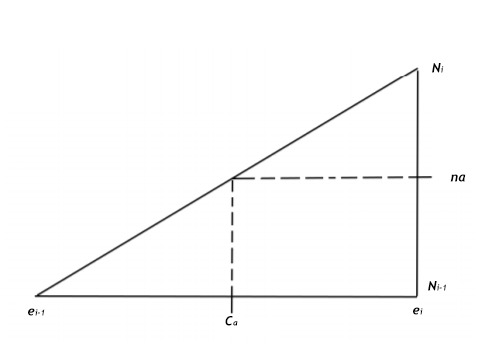
\includegraphics[scale=0.7]{imagenes/triangulo_ejer_9.jpeg}
\end{figure}

  $$\frac{a_{i}}{c_{\alpha}-e_{i-1}} = \frac{n_{i}}{n\alpha - N_{i-1}} \longleftrightarrow C_{\alpha} = e_{i-1} + \frac{n\alpha - N_{i-1}}{n_{i}}\alpha_{i}$$
Esta fórmula será usada de aquí en adelante en los ejercicios.
\[
C_{0.40} = 4 + \frac{0.4 \cdot 498 -245}{81}\cdot 1 = 3.435 \hspace{0.2cm} Se \hspace{0.1cm} suspende \hspace{0.1cm} por \hspace{0.1cm} debajo \hspace{0.1cm} de \hspace{0.1cm} dicha \hspace{0.1cm} nota.
\]

Para el cálculo de la nota máxima en aprobados, notables, sobresalientes, y matrículas hemos de emplear la fórmula obtenida: \\

Aprobados \(\Rightarrow\) cuantil 0.70 \(\Rightarrow n \cdot 0.7= 348.6 \Rightarrow\) La nota máxima de los aprobados está en el intervalo (5,6].

\[
C_{0.70} = 6 + \frac{348.6 - 409}{70} \cdot 1 = 5.137142857
\]

Notables \(\Rightarrow\) Cuantil 0.85 \(\Rightarrow n \cdot 0.85 = 423.3 \Rightarrow\) Buscar en (6,7].

\[
C_{0.85} = 7 + \frac{423.3 - 450}{41} \cdot 1 = 6.349
\]

Sobresalientes \(\Rightarrow\) Cuantil 0.95 \(\Rightarrow n \cdot 0.95 = 473.1 \Rightarrow\) Buscar en (7,8].

\[
C_{0.95} = 8 + \frac{473.1 - 478}{28} \cdot 1 = 7.825
\]

Matrículas \(\Rightarrow\) Es obvio, pues el cuantil 1 es \(C_{1} = 10\)
\end{ej}
\bigskip
\begin{ej}
Se ha medido la altura de 110 jóvenes, obteniendo:

\begin{center}
    \begin{tabular}{|c|c|c|c|c|c|}
    \hline
    Altura & (1.55, 1.60] & (1.60, 1.70] & (1.70, 1.80] & (1.80, 1.90] & (1.90, 2.00] \\
    \hline
    Nº jóvenes & 18 & 31 & 24 & 20 & 17 \\
    \hline
     $N_{i}$ & 18 & 49 & 73 & 93 & 110 \\
    \hline
    $a_{i}$ & 0.05 & 0.1 & 0.1 & 0.1 & 0.1 \\
    \hline
    \end{tabular}
\end{center}

\bigskip
\textbf{Conceptos:}
\begin{center}
    \fbox{
    \begin{minipage}[h!]{1\linewidth}
    \begin{itemize}
        \item Población\label{poblacion}: jóvenes
        \item Tamaño de la población: \(n = 110\)
        \item Variable estadística (X): altura de cada joven
        \item Modalidades: intervalos de distinta amplitud que van de 1.55 a 2.00; (5 modalidades)
    \end{itemize}
    \end{minipage}
    }
\end{center}
\bigskip

\begin{enumerate}[label=\textit{\alph*)}]
    \item Si se considera bajos al 3\% de los individuos de menor altura, ¿cuál es la altura máxima que pueden alcanzar?
    \\\\
    Para poder saberlo, es necesario calcular el cuantil $0.03$, que indica la altura por debajo de la cual se halla el $3\%$ de la población estudiada. Deduzcamos la fórmula para los cuantiles:
  \\ 
  $1 \ n\alpha = 3.3 \leftarrow$ Como $N_{1} = 18$ es inmediatamente mayor que $n\alpha$, $C_{0.03}$ ha de hallarse en el intervalo $(155,160]$. \\
    $2$ Si tomamos el tramo de la curva de distribución de $I_{i}$ 
    \\
    Empleamos la formula para $C_{0.03}$ 
    $$C_{0.03} = 1.55 + \frac{3.3 - 0}{18}0 0.05 = 1.5591\wideparen{6} \approx 1.56 m$$
    \item Si se condiera altos al 18\% de los individuos de mayor altura, ¿cuál es su altura mínima? \\\\
    Debemos calcular la altura por debajo de la cual queda el $82\%$ de la población. Repitiendo el proceso anterior empleando la fórmula: 
    \\
    1 $n\alpha=90.2 \implies N_{y} = 93$ es inmediatamente mayor que $n\alpha$, $C_{0.82}$ ha de hallarse $I_{y}$:
    $$C_{0.82} = 1.80 + \frac{90.2 - 73}{20}0.1 = 1.886$$
    \item ¿Qué altura es superada sólo por 1/4 de los jóvenes? \\\\
    Como el $\frac{3}{4}$ de los jóvenes no superan esa altura y $\frac{3}{4}=0.75$, hemos de calcular $C_{0.75}$:
    \\
    1 $n\alpha = 82.5 \implies C_{0.75}$ ha de hallarse en $I_{4}$:
    $$C_{0.75} = 1.80 + \frac{82.2 - 73}{20}0.1 = 1.848$$
    \item Calcular el número de jóvenes cuya altura es superior a 1.75. \\\\
    En este caso sería hacer el cuantil inverso, es decir, deducir qué cuantil cumple que $C_{\alpha} = 1.75$ y finalmente calcular $n\alpha$ . Deduciendo que está en $I_{3}$, empleemos la fórmula:
    $$1.75 = 1.75 + \frac{110\alpha - 49}{24}0.1 \longleftrightarrow \alpha = 0.5\wideparen{54}$$
    $n\alpha = 110 \cdot 0.5\wideparen{54} = 61$ jóvenes no superan dicha altura y, por tanto, $49$ la superan. \\
    \item Calcular la altura máxima de los 11 jóvenes más bajos.\\\\
    $\frac{11}{110} = 0.1 \ \implies$ Se nos pide el cuantil $0.1$, $C_{0.1}$, que se halla en $I_{1}$: \\
    $C_{0.1} = 1.55 + \frac{11-0}{18}0.05 = 1.580\wideparen{5} \approx 1.58$ m. \\
    \item Calcular la altura mínima de los 11 jóvenes más altos.
    \\\\
    $1-\frac{11}{100}=0.9 \implies$ Se nos pide la altura por debajo de la cual se encuentra el $90\%$ de la población, es decir, $C_{0.9}$, que se halla en $I_{5}$: \\
    $$C_{0.9} = 1.90 + \frac{99-93}{17}0.1 = 1.935 \ m$$
\end{enumerate}
\end{ej}

\begin{ej}
Realizando una prueba para el estudio del cáncer a 150 personas se obtuvo la siguiente tabla según la edad de los enfermos:

\begin{center}
    \begin{tabular}{|c|c|c|c|c|c|}
    \hline
         Edad & (10, 30] & (30, 40] & (40, 50] & (50, 60] & (60, 90]  \\
         \hline
         Nº enfermos & 15 & 22 & 48 & 40 & 25 \\ 
         \hline
    \end{tabular} \\
    \end{center}
    
    \bigskip
    
\textbf{Conceptos:}
\begin{center}
    \fbox{
    \begin{minipage}[h!]{1\linewidth}
    \begin{itemize}
        \item Población\label{poblacion}: enfermos de cáncer
        \item Tamaño de la población: \(n = 150\)
        \item Variable estadística (X): edad de cada enfermo
        \item Modalidades: intervalos de distinta amplitud que van de 10 a 90; (5 modalidades)
    \end{itemize}
    \end{minipage}
    }
\bigskip

    \begin{tabular}{|c|c|c|c|c|c|c|c|c|c|} 
    \hline
         Edad & $n_{i}$ & $a_{i}$ & $h_{i}$ & $N_{i}$ & $C_{i}$ & $n_{i}c_{i}$ & $n_{i}c_{i}^2$ & $n_{i}c_{i}^3$ & $n_{i}c_{i}^4$ \\
         \hline
         (10,30] & 15 & 20 & 0.75 & 15 & 20 & 300 & 6000 & 120000 & 2400000\\ 
         \hline
         (30,40] & 22 & 10 & 2.2 & 37 & 35 & 770 & 26950 & 943250 & 33013750\\ 
         \hline
         (40,50] & 48 & 10 & 4.8 & 85 & 45 & 2160 & 97200 & 4374000 & 19683000\\ 
         \hline
         (50,60] & 40 & 10 & 4 & 125 & 55 & 2200 & 121000 & 6655000 & 366025000\\ 
         \hline
         (60,90] & 25 & 30 & $0.8\wideparen{3}$ & 150 & 75 & 1875 & 140625 & 10546875 & 791015625\\ 
         \hline
         & 150 & & & & & 7305 & 391775 & 22639125 & 1389284375 \\ 
         \hline
    \end{tabular}
\end{center}

\begin{enumerate}[label=\textit{\alph*)}]
    \item Calcular la edad más común de los individuos estudiados. \\
    Se nos está pidiendo la moda, la cual la encontraremos en el intervalo modal, es decir, el intervalo con mayor densidad de frecuencia $h_{i} = \frac{n_i}{a_i}$

 $\frac{n_{i}}{a_{i}}$. En este caso, $h_{3} > h_{j} \ \forall j \not = 3$ con $j \in \ \{1,\dots,5\}$. Ahora llevamos a cabo la semejanza de triángulos vista en clase sobre un trozo del histograma (el intervalo modal y sus contiguos): \\
    
    \begin{figure}[h!]
    \centering
    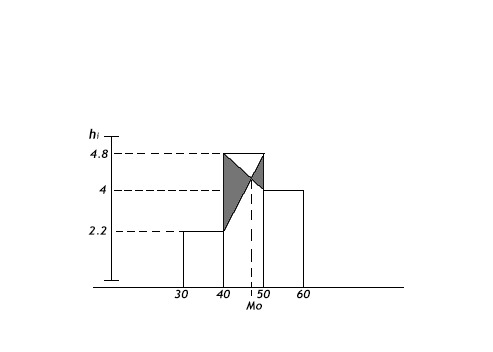
\includegraphics[scale=0.7]{imagenes/grafica_moda.jpeg}
	\end{figure}
	
    Con los triángulos semejantes, usaremos la razón base entre altura (el dibujo no está a escala): \\
    $$\frac{4.8-2.2}{Mo - 40} = \frac{4.8 - 4}{50 - Mo} \longleftrightarrow Mo= 47.647 \ \text{años} $$
    \item Calcular la edad mínima y máxima del 30\% central de los individuos.\\
    
    \begin{figure}[h!]
    \centering
    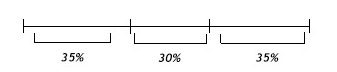
\includegraphics[scale=2.5]{imagenes/30_central_ej_10.jpeg}
	\end{figure}

    Lo que se nos pide es equivalente a calcular $C_{0.35}$ y $C_{0.65}$. Emplearemos la fórmula demostrada en el ejercicio 8: \\
    1 $n\alpha = 150\cdot0.35 = 52.5 \implies \ C_{0.35}$ estará en $I_{3}$ pues $N_{3}$ es inmediatamente mayor que $n_{\alpha}$ \\
    $$C_{0.35} = 40 + \frac{52.5 - 37}{48} \cdot 10 = 43.22291\wideparen{6} \text{ años (edad mínima)}$$
    Y para el cuantil $C_{0.65}$:\\
    1 $n\alpha = 150\cdot0.65 = 97.5 \implies$ Estará en $I_{4}$ ya que $N_{4}$ es inmediatamente superior a $n\alpha$
    $$C_{0.65} = 50 + \frac{97.5 - 85}{40} \cdot 10 = 53.125 \text{ años (edad máxima)}$$
    \item Calcular el recorrido intercuartílico y la desviación típica.\\
    $R_{I} = Q_{3} - Q_{1} \implies$ Necesitamos hallar los cuartiles 1 y 3 que equivalen a los cuantiles $0.25$ $0.75$. Repetimos el proceso del anterior apartado: \\
    1 $n\alpha = 150 \cdot 0.25 = 37.5 \implies C_{0.25}$ estará en $I_{3} = (40,50]$ pues $N_{3}$ es inmediatamente mayor que $37.5$
    $$C_{0.25} = 40 + \frac{37.5-37}{48} \cdot 10 = 40.1041\wideparen{6} \text{ años}$$
    1 $n\alpha = 150 \cdot 0.75 = 112.5 \implies C_{0.75}$ estará en $I_{4} = (50,60]$ pues $N_{4}$ es inmediatamente mayor que $112.5$
    $$C_{0.75} = 50 + \frac{112.5-85}{40} \cdot 10 = 56.875 \text{ años}$$
    Por lo tanto, $R_{I} = Q_{3} - Q_{1} = 56.875 - 40.1041\wideparen{6} = 16.7708\wideparen{3} \text{ años}$ \\
    Esto significa que todos los datos encontrados en el 50\% central de la distribución se diferencian como máximo en $16.7708\wideparen{3} \text{ años}$. \\ 
    En cuanto a la desviación típica, debemos hallar antes la varianza: 
    $$\sigma^2 = \frac{1}{n} \sum_{i = 1}^k n_{i}c{i}^2 - \bar{x}^2 = \frac{1}{n} \sum_{i = 1}^k n_{i}c{i}^2 - (\frac{1}{n} \sum_{i = 1}^k n_{i}c{i})^2 = \frac{391775}{150}- (\frac{7305}{150})^2 = 240.1434 \text{ años al cuadrado}$$
    $\sigma = +\sqrt{\sigma^2} = 15.49656$ años $\implies$ Esto significa que la mayoría de los datos de nuestra distribución se hallan en el intervalo $[\bar{x}-\sigma, \bar{x} + \sigma]$.
    \item Calcular e interpretar los valores de los coeficientes de asimetría y curtosis. \\
    

    \fbox{
    \begin{minipage}[h!]{1\linewidth}
    \begin{itemize}
        \item Momentos: son indicadores genéricos de una distribución. Se basan en una generalización de la idea de media. Si dos distribuciones son iguales todos sus infinitos momentos coinciden. \\ Momento de orden $r$ respecto al valor $a$:\qquad sea $r$ un número real positivo 
        \[\prescript{}{a}{m}_{r} = \sum_{i=1}^{k} f_{i}(x_{i} - a)^{r} = \frac{1}{n}\sum_{i=1}^{k} n_{i}(x_{i} - a)^{r}\]
        \begin{itemize}
            \item Momentos no centrales: momentos respecto del origen; $a=0$
            \[m_r = \sum_{i=1}^{k} f_i x_i^r\]
            \item Momentos centrales: momentos respecto de la media aritmética; $a=\overline{x}$
            \[\mu_r = \sum_{i=1}^{k} f_{i}(x_{i} - \overline{x})^{r}\]
        \end{itemize}
        \item Medidas de asimetría: sea $X$ una variable estadística, se entiende por asimetría de $X$ a la falta de simetría respecto del eje vertical $x = \overline{x}$. Una distribución es simétrica si la perpendicular que pasa por la media aritmética divide al diagrama diferencial (histograma, en el caso continuo; o diagrama de barras, en el discreto) en dos partes iguales; de lo contrario, es asimétrica.
        \begin{itemize}
            \item Coeficiente de asimetría de Fisher,  $\gamma_{1}(x)$
            \item Coeficientes de asimetría de Pearson,  $A_{p}$ , $A_{p^*}$
            \begin{itemize}
                \item $coeficiente > 0 \Rightarrow$ distribución asimétrica por la derecha o positiva
                \item $coeficiente < 0 \Rightarrow$ distribución asimétrica por la izquierda o negativa
                \item $coeficiente = 0 \Rightarrow$ distribución simétrica
                \end{itemize}
        \end{itemize}
        \item Medidas de apuntamiento o curtosis: miden la menor o mayor concentración central de frecuencias de una distribución respecto a la que presenta una distribución Normal de su misma media y su misma desviación típica.
        \begin{itemize}
            \item Coeficiente de curtosis de Fisher,  $\gamma_{2}(x)$
            \item Coeficiente de curtosis de Kelley,  $K$
            \begin{itemize}
                \item $coeficiente > 0 \Rightarrow$ distribución leptocúrtica
                \item $coeficiente < 0 \Rightarrow$ distribución platicúrtica
                \item $coeficiente = 0 \Rightarrow$ distribución mesocúrtica
            \end{itemize}
        \end{itemize}
    \end{itemize}
    \end{minipage}
    }

\bigskip
    
    De asimetría son 3: \\
  
    - De Fisher: $\rightarrow  \gamma_{1}(x) = \frac{\mu_{3}}{\sigma_{x}^3}$ \\
    \\
    - De Pearson: 
    $$A_{p} = \frac{\bar{x}-Mo}{\sigma_{x}}$$
    $$A_{p^*} = \frac{3(\bar{x}-Me)}{\sigma_{x}}$$
    \\
    $$\mu_{3} = m_{3} - 3m_{2}m_{1} + 2m_{1}^3 = \frac{1}{n} \sum n_{i}c{i}^3 - 3\frac{1}{n}\sum n_{i}c{i}^2 \cdot \bar{x} + 2\cdot \bar{x}^3 =$$
    $$= \frac{22639125}{150} - \frac{3}{150} \cdot 391775 \cdot \frac{7305}{150} + 2 \cdot (\frac{7305}{150})^3 = 341.256$$
    $$\gamma_{1}(x) = \frac{\mu_{3}}{\sigma_{x}^3} = \frac{341.256}{15.49656^3}= 0.0917 > 0 \implies \text{ Es algo asimétrica por la derecha}$$
    $$A_{p} = \frac{\bar{x}-Mo}{\sigma_{x}} = \frac{\frac{7305}{150}-47.647}{15.49656} = 0.06795$$
    Para $A_{p^*}$ nos falta Me: \\
    1 $n\alpha = 150 \cdot 0.5 = 75 \implies$ Me estará en $I_{3}$ \\
    $$Me = 40 + \frac{75 - 37}{48}\cdot 10 = 47.91\wideparen{6}$$
    $$A_{p^*} = \frac{3(\bar{x}-Me)}{\sigma_{x}} = \frac{3\cdot(\frac{7305}{150}-47.91\wideparen{6})}{15.49656} = 0.151647$$
    \\
    Ahora pasamos a los coeficientes de Curtosis: \\
    \\
    - Fisher: $\gamma_{2(x)} = \frac{\mu_{4}}{\sigma^4}-3$ \ Hallemos $\mu_{4} = m_{4} - 4m_{3}m_{1}+6m_{1}^2m_{2}-3m_{1}^4$: \\
    $$\mu_{4}=\frac{1}{n}\sum n_{i}c_{i}^4-4\frac{1}{n} \sum n_{i}c_{i}^3\cdot \bar{x}+6\bar{x}^2\cdot\frac{1}{n} \sum n_{i}c_{i}^2 - 3\bar{x}^4 = $$
    $$= \frac{1389284375}{150}-4 \cdot\frac{1}{150}\cdot(22639125)\cdot\frac{7305}{150} + 6\cdot(\frac{7305}{150})^2\cdot\frac{1}{150}\cdot 391775 - 3\cdot (\frac{7305}{150})^4 =153232.46$$
    $$\gamma_{2}(x) = \frac{\mu_{4}}{\sigma^4} - 3=\frac{153232.46}{15.49656^2} - 3 = -0.3429 < 0$$
    La distribución es platicúrtica, es decir, presenta una menor concentración central de frecuencias que una normal de su misma media y desviación típica (está más aplanada que la curva normal y los datos están más dispersos). \\
    De Kelley: $\frac{1}{2} \cdot \frac{Q_{3}-Q_{1}}{D_{9}-D_{1}} - 0.263$, como ya tenemos $Q_{1}$ y $Q_{3}$, debemos calcular $D_{1} =  C_{0.1}$ y $D_{9} = C_{0.9}$: \\
    1 $n\alpha = 15 \implies C_{0.1}$ coincide justamente con el extremo superior de $I_{1} = (10,30]$, es decir, 30 años. \\
    1 $n\alpha = 135 \implies C_{0.9}$ ha de hallarse en $I_{5} = (60,90]$ ya que $N_{5}$ es inmediatamente mayor que 135. Aplicamos la fórmula demostrada: \\
    $$C_{0.9} = 60 + \frac{135 -125}{25}\cdot30 = 72 \text{ años}$$
    $$K = \frac{1}{2} \cdot \frac{Q_{3}-Q_{1}}{D_{9}-D_{1}} - 0.263 = \frac{1}{2} \cdot \frac{56.875-40.4041\wideparen{6}}{72-30} - 0.263 = -0.06335 < 0$$
    Como $K<0$, la distribución es platicúrtica, por lo que llegamos a la misma conclusión que con el coeficiente de curtosis de Fisher.
\end{enumerate}
\end{ej}

\end{document}